\usepackage{array}
\usepackage{booktabs}
\usepackage{xcolor}
\usepackage{colortbl}

\section{Stage 2: Orchestrator} \label{sec:work_stage2_orchestrator}

\begin{figure}[htbp]
  \centering
  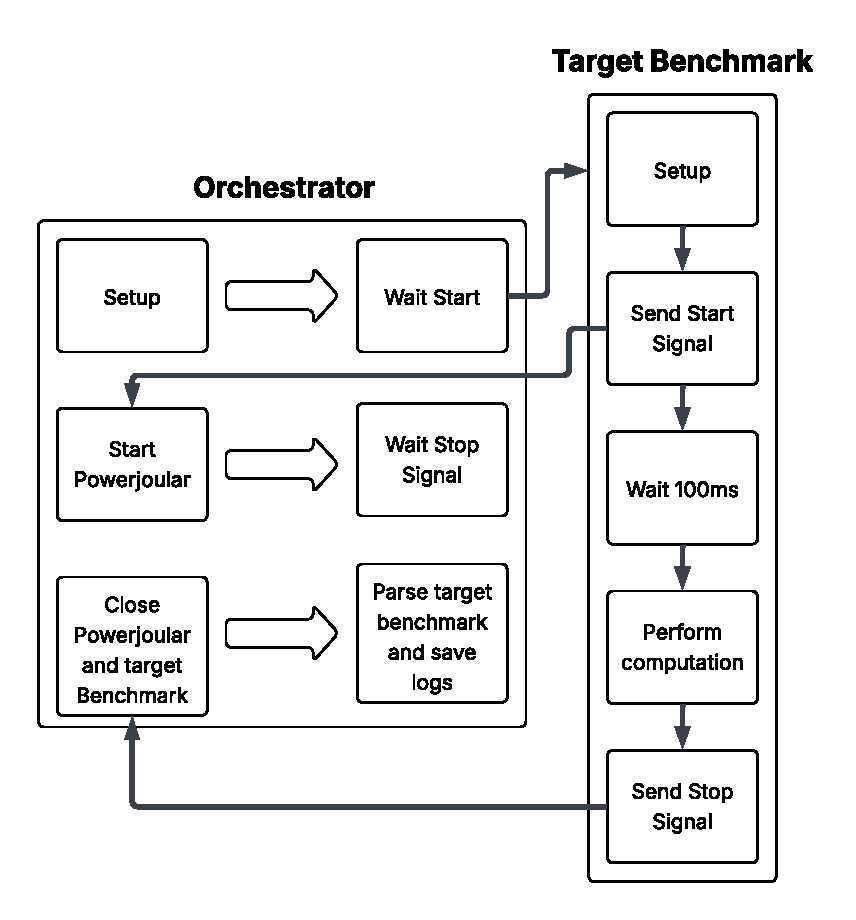
\includegraphics[width = 1 \textwidth]{figures/orchestrators_process.pdf}
  \caption{Orchestrator Workflow}
  \label{fig:orchestrators_process}
\end{figure}


Having all the programs generated, it is possible to move to the next stage. Gathering the energy profiles for each of the generated programs. This step is necessary, of course, because to give energy consumption estimates, first it is necessary to obtain energy profiles~\cite{10.1145/2884781.2884869,8816747}, so the machine learning models can obtain the most accurate results possible. To make this task as easily as possible, a process was implemented, so the task was made automatically, taking into account what was said in \ref{sec:background_benchmarking}. 

Note: Although this part was developed chronologically before Section \ref{sec:work_stage1_program_generator}, it is presented as Stage 2 to reflect the logical structure of the system: programs must first be generated before they can be energy profiled. For this reason, the program generator templates are designed to integrate directly with the orchestrator.

As described in \ref{sec:background_energy} there are several tools capable of performing dynamic energy measurements. In our case we choose PowerJoular, it has good features that caught our attention, for example being a command line tool that could be easily integrated in almost every programming language, it stores the energy used in a CSV file (easy to work with), capable of only reading energy of running processes and so on, as explained before. So, PowerJoular is the tool that will measure the energy of our programs.

Since PowerJoular is a command line tool, it is launched as a process, and then it can be killed whenever needed because it is a process as well. This allows to measure not only programs/processes energies but have a more precise measurement, as it is possible to call PowerJoular to measure a specific computation and then kill it when the computation is finished.

With all of this in mind a process was built. The process uses an orchestrator that is responsible for invoking the target program and the measurement tool (PowerJoular) to accurately measure the energy consumption of the program or the specific computation being analyzed within it.

In the program generator it was shown an example of a template \ref{lst:template_example}. This structure was carefully crafted in order to work with the orchestrator.



When measuring energy, there is a particular problem with computation. It is too fast. It is really difficult to measure a single operation of, for example, a List.add(Object) with most tools, as it simply to fast for the tool to capture, and if the tool was able to capture it, the energy measured would have too much noise to be considered. So, it surges the need to loop through the method until the tool (PowerJoular) is capable of getting its energy and then dividing the total energy by the number of times it looped. This can work, but it brings other errors that will need to be considered.

If we approach the measurements with the loop technique, first we need to create the variables needed for the method target to analysis, like shown in \ref{lst:var_placeholders}. But there is a problem, the methods are treated like a black box, it is not possible to know what the methods are going to do with the parameters or with its variables, for example, the method List.size() it receives nothing, and return the size of the list which is fine. However, this raises problems with other methods, such as List.add(Object), maybe not in the first iterations. But what if the loop iterates too many times? It will make the list much bigger than the initial list, which again will cause differences in the energy measurements and later in the energy predictions. 
Now, suppose we have a custom method called sort that takes a randomly ordered list and sorts it. This introduces a problem when measuring its energy consumption. On the first run, the method will sort the unsorted list, which may take significant time depending on the randomness of the data and the sorting algorithm used. However, on subsequent runs with the same list, the input is already sorted, meaning the sort method will likely complete much faster or with minimal effort. This difference can result in misleading or inconsistent measurements.

\begin{figure}[htbp]
  \centering
  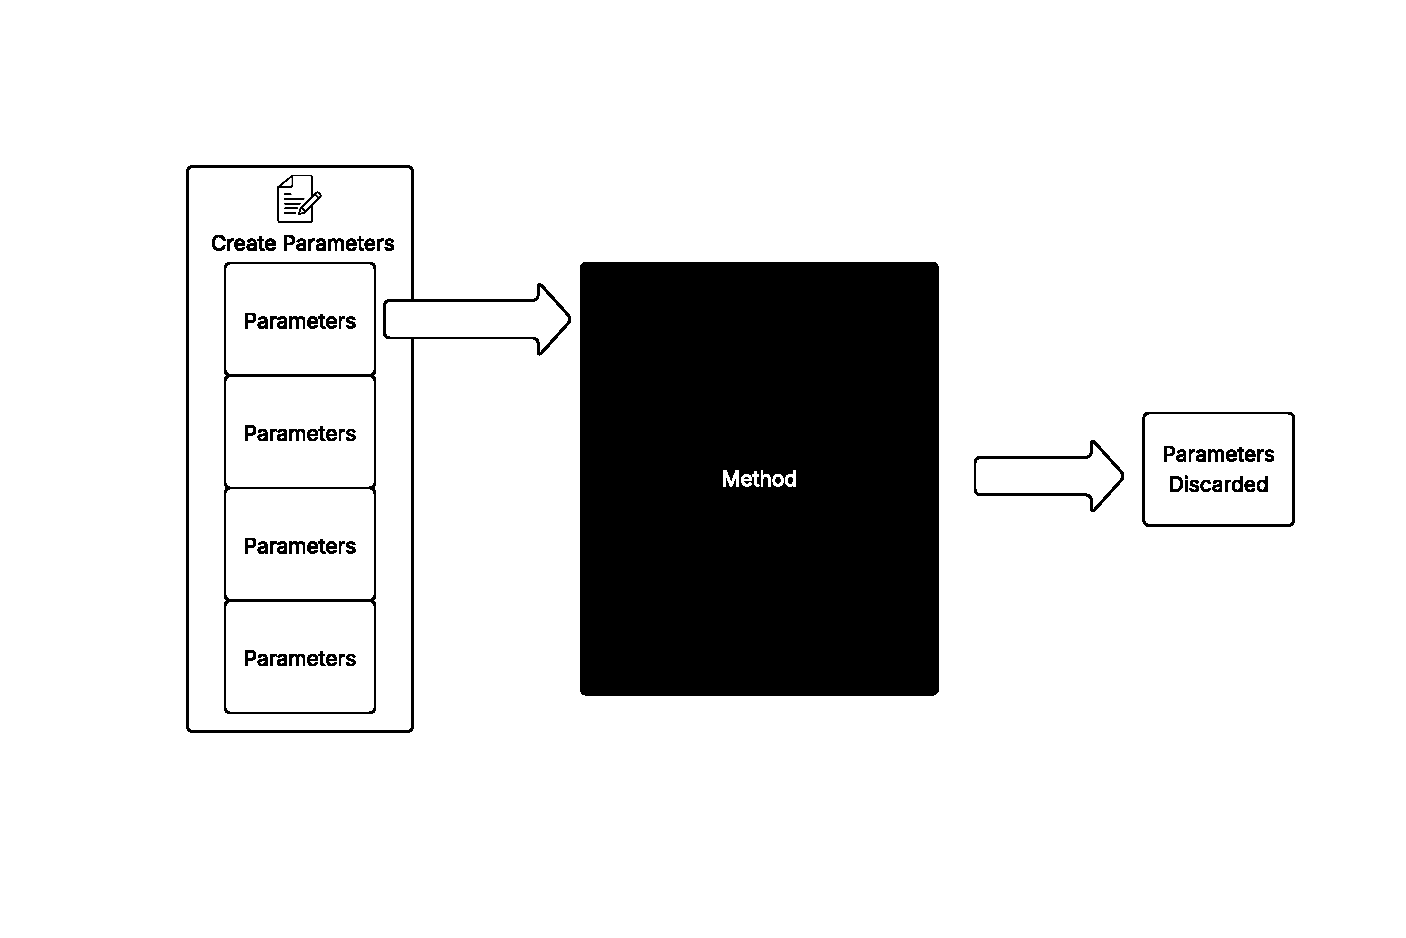
\includegraphics[width = 1 \textwidth]{figures/array.pdf}
  \caption{Array example}
  \label{fig:array}
\end{figure}

To prevent this from happening the approach used was to create an array that holds the parameters \ref{fig:array}. Basically, the parameters are created into an array, all with the same values, but with different references. Now, if one of the elements is changed during its execution on the method, it will not affect the other's execution. Of course, since now there are multiple references of the same values, the memory usage is much higher, so that is why there is an array size, also empirically chosen, to avoid memory errors and avoid having the array so small the PowerJoular would not have time to perform the measurements. There are, for now, 3 different array sizes (75_000, 100_000, 150_000). PowerJoular by default needs to run for 1 second to create the CSV file that has the energy used for the target process, so these sizes aim so that looping the array takes at least a second. In some cases, the CSV file may not be generated because the loop executes too quickly. In such instances, the energy reading will be assumed to be 0 J, as the execution was too fast to record a value. Using an array in this case is preferable to a list, as it introduces less overhead and has a smaller impact on energy measurements.


\begin{listing}[H]
\begin{minted}[linenos, fontsize=\small, frame=none, bgcolor=white,breaklines=true,breakanywhere=true]{java}
private static int computation(BenchmarkArgs[] args, int iter) {
        int i = 0;
        while (!TemplatesAux.stop && i < iter) {
              arrayList_add_java_lang_Object_(args[i].var0, args[i].var1);
               i++;
        }
        return iter;
    }
\end{minted}
\caption{Computation method}            
\label{lst:Computation_method}
\end{listing}

The computation method shown in Listing \ref{lst:Computation_method} illustrates how each profiling method operates independently of the specific method being evaluated. It attempts to execute the target function repeatedly for approximately one second. In this particular case, the target function performs the operation \texttt{var.add(arg0);} and returns the number of iterations completed, which is then used for further calculations.


With the process structure now defined, we can proceed to explain how it functions.

The workflow of this step can be described as follows:

\begin{itemize}
  \item The orchestrator launches a command to start the target Java Program and waits a signal.
  \item The Java program starts and setup the necessary elements to run (creating all the variables, reading/writing files, populating the array, etc.) and then before starting the computation it wants to measure, it sends a start signal to the orchestrator to start monitoring, and waits for 100 milliseconds.
  \item The orchestrator receives the start signal and reads the PID, which is stored in a file during the target program setup. Finally, it starts PowerJoular using that PID. Then it waits for the stop signal.
  \item The Java program will run until it finishes the computation. The computation runs for a maximum of one second. Then the number of iterations are stored in a file and the stop signal is sent back to the orchestrator.
  \item The orchestrator on receiving the stop signal, first stops PowerJoular and then stops the target program, if needed. Then it parses the target program to extract its features, combines them with the energy information stored in the files created by PowerJoular, stores it in a CSV file.
\end{itemize}

All these steps are performed for each generated program. At the end of the process, a log file is created containing key information, including all the programs used, the PowerJoular files generated, temporary files, error logs, and features.

The features extracted from the parser can be seen in the table \ref{tab:features_extracted}

\begin{table}[htbp]
\centering
\caption{Features extracted}
\label{tab:features_extracted}
\begin{tabular}{||l|c||}
\hline\hline
\textbf{Feature Name} & \textbf{Description} \\
\hline\hline
VariableDeclarations & Number of variable declarations in the code. \\
\hline
Assignments & Number of assignment operations (=) in the code. \\
\hline
BinaryOperators & Number of binary operators used (e.g., +, -, *, /, \&\&). \\
\hline
MethodInvocations & Number of method calls in the code. \\
\hline
CustomMethodsUsed & Number of user-defined (custom) methods used in the code. \\
\hline
CustomObjectsUsed & Number of user-defined (custom) objects used in the code. \\
\hline
BranchCount & Number of branching statements ( if, else if, else ) in the code. \\
\hline
LoopCount & Number of loops ( for, while, do-while ) in the code. \\
\hline
LoopMaxDepth & Maximum nesting depth of loops in the code. \\
\hline
CyclomaticComplexity & The cyclomatic complexity of the code (number of independent execution paths). \\
\hline
LiteralCount & Number of literals (numbers, strings, boolean values) in the code. \\
\hline
VariableCount & Total number of variables in the code. \\
\hline
Reassignments & Number of times variables are reassigned a new value. \\
\hline
VariableTypes & Types of variables used (e.g., int, String, List$<$String$>$). \\
\hline
ImportsUsed & List of imported Java packages/libraries in the code. \\
\hline
java.langMethodUsed & If the method is from java.lang, the specific function name (e.g., ArrayList.get). \\
\hline
Inputs & The parameters received by the method. \\
\hline\hline
\end{tabular}
\end{table}